\section{MPLS Signatures Validation}\label{validation}
% %%%%%%%%%%%%%%%%%%%%%%%%%%%%%%%%%%%%
\begin{figure}[!t]
  \begin{center}
    \subfigure[qTTL signature.]{\label{validation.qTTLFig}
      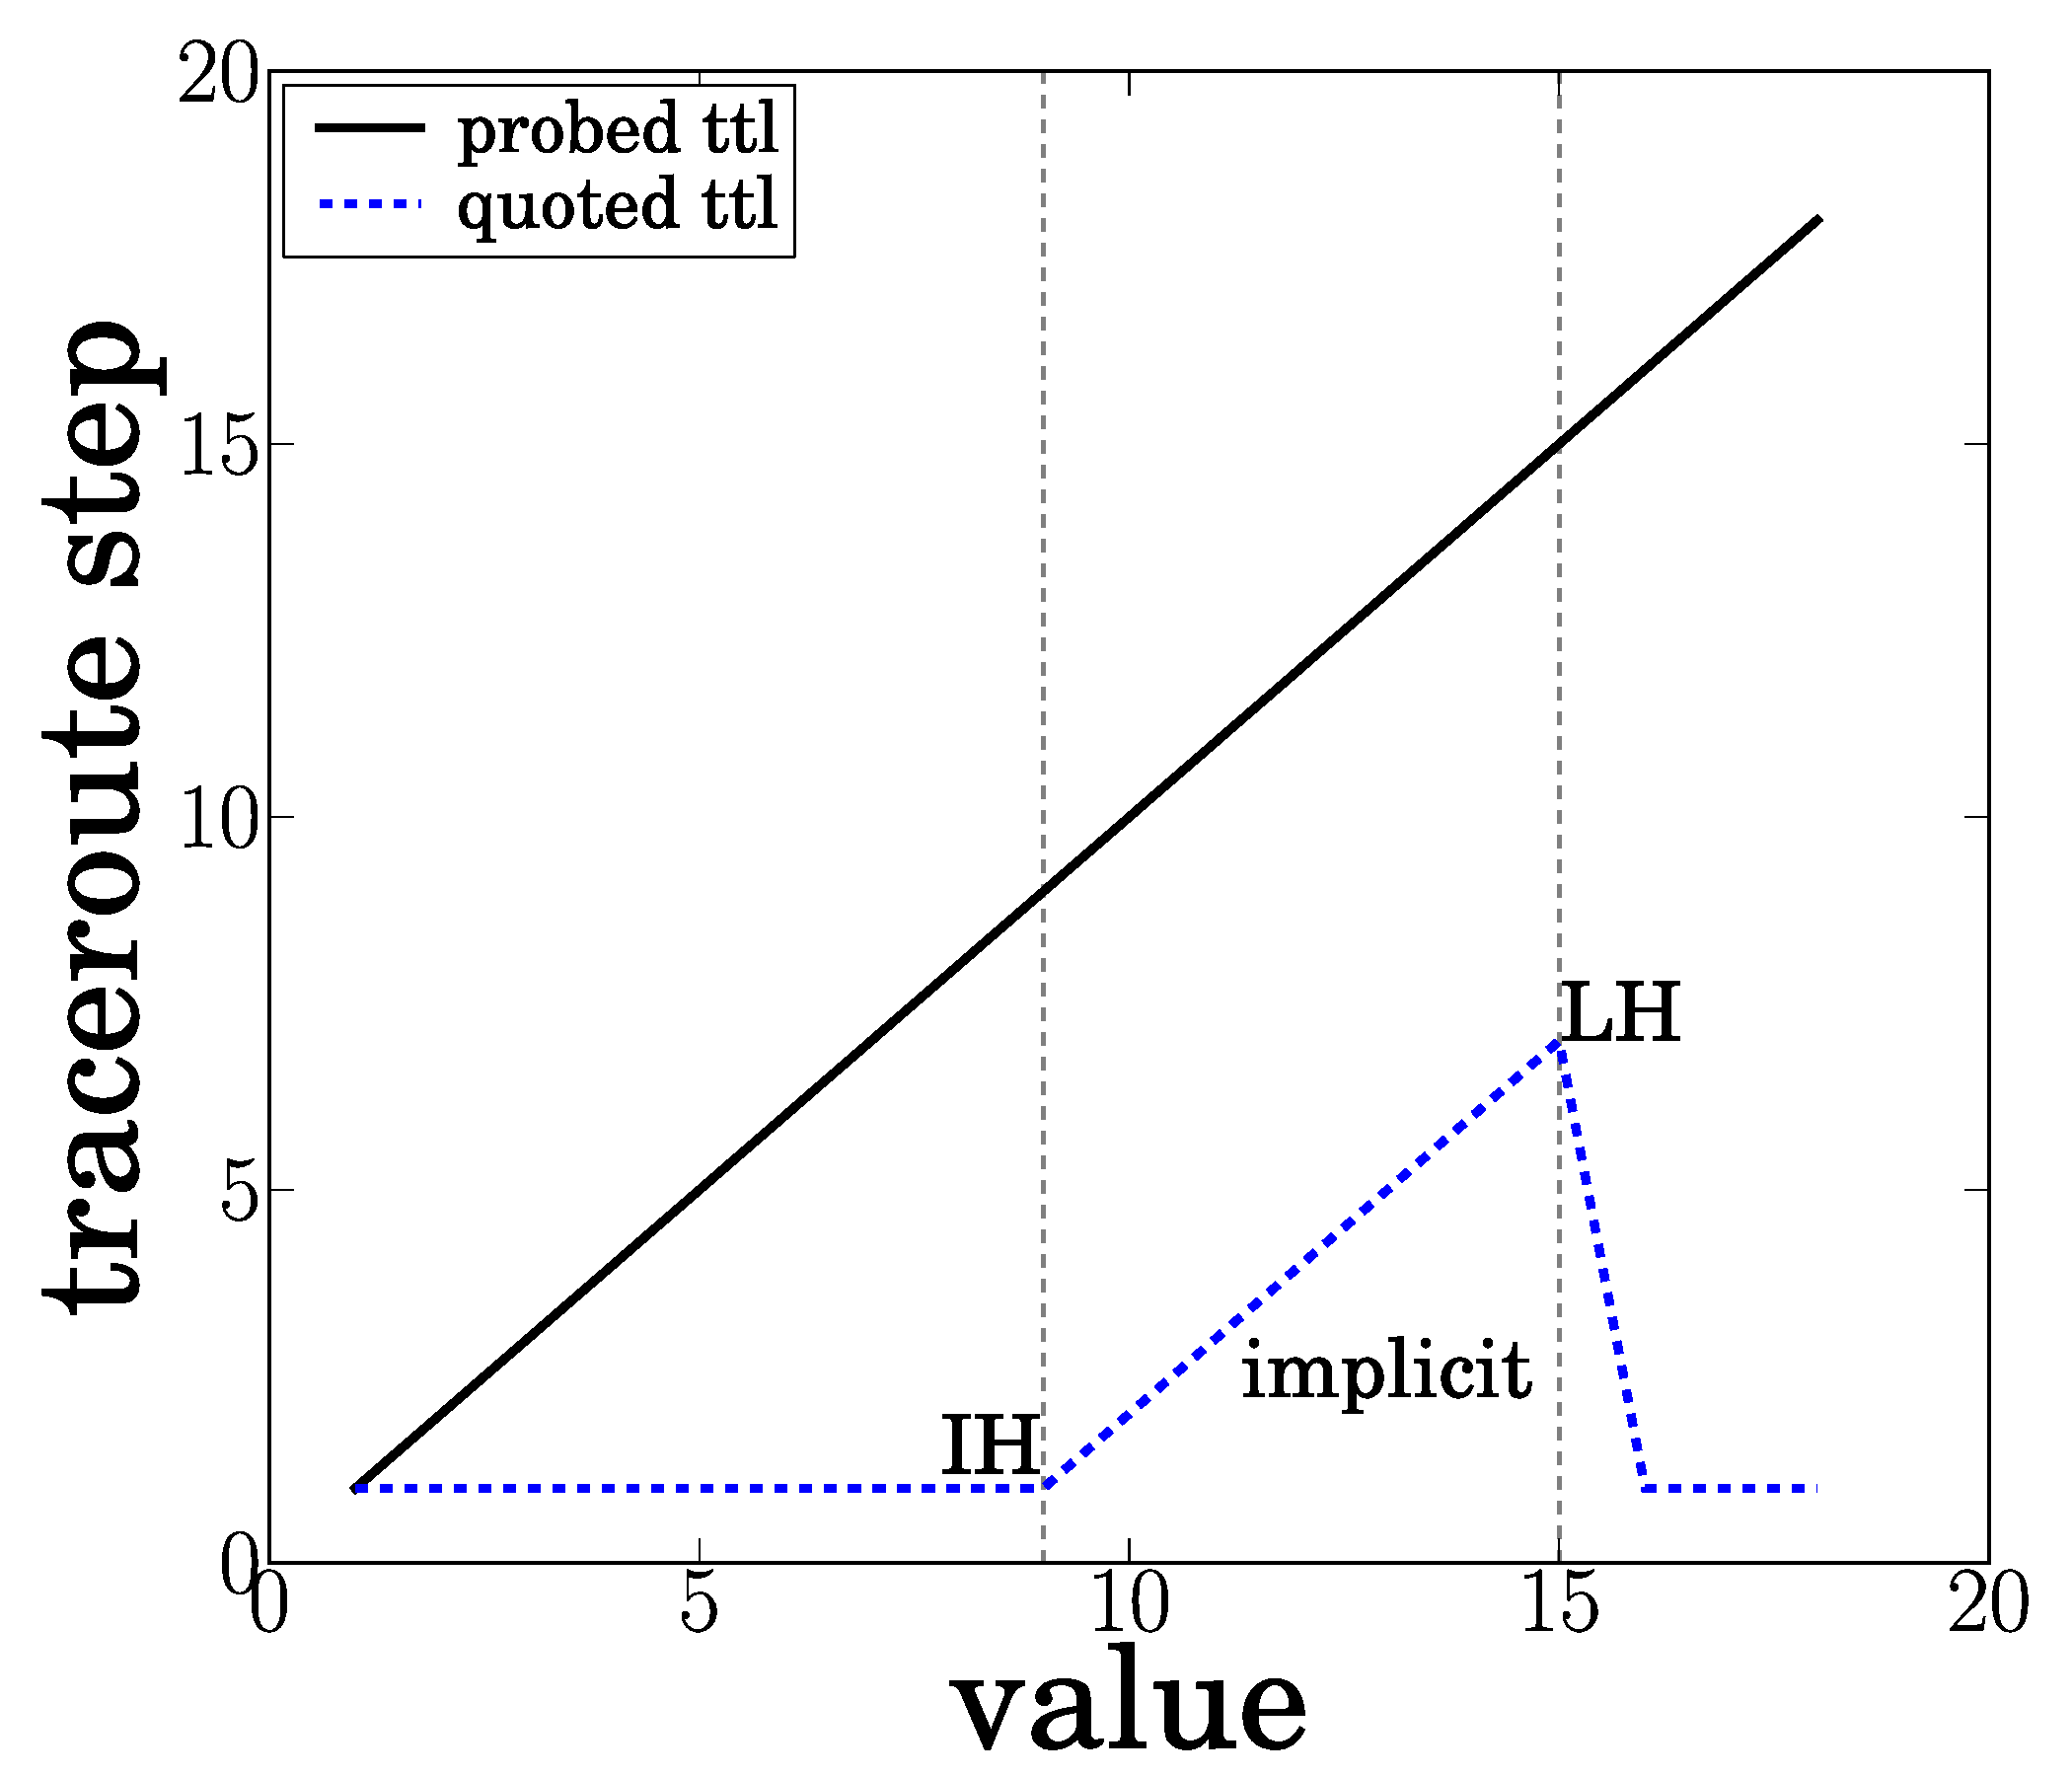
\includegraphics[width=4cm]{QuotedTTL}}
\hspace{-0.3cm}      
    \subfigure[u-turn signature.]{\label{validation.uturn1Fig}
      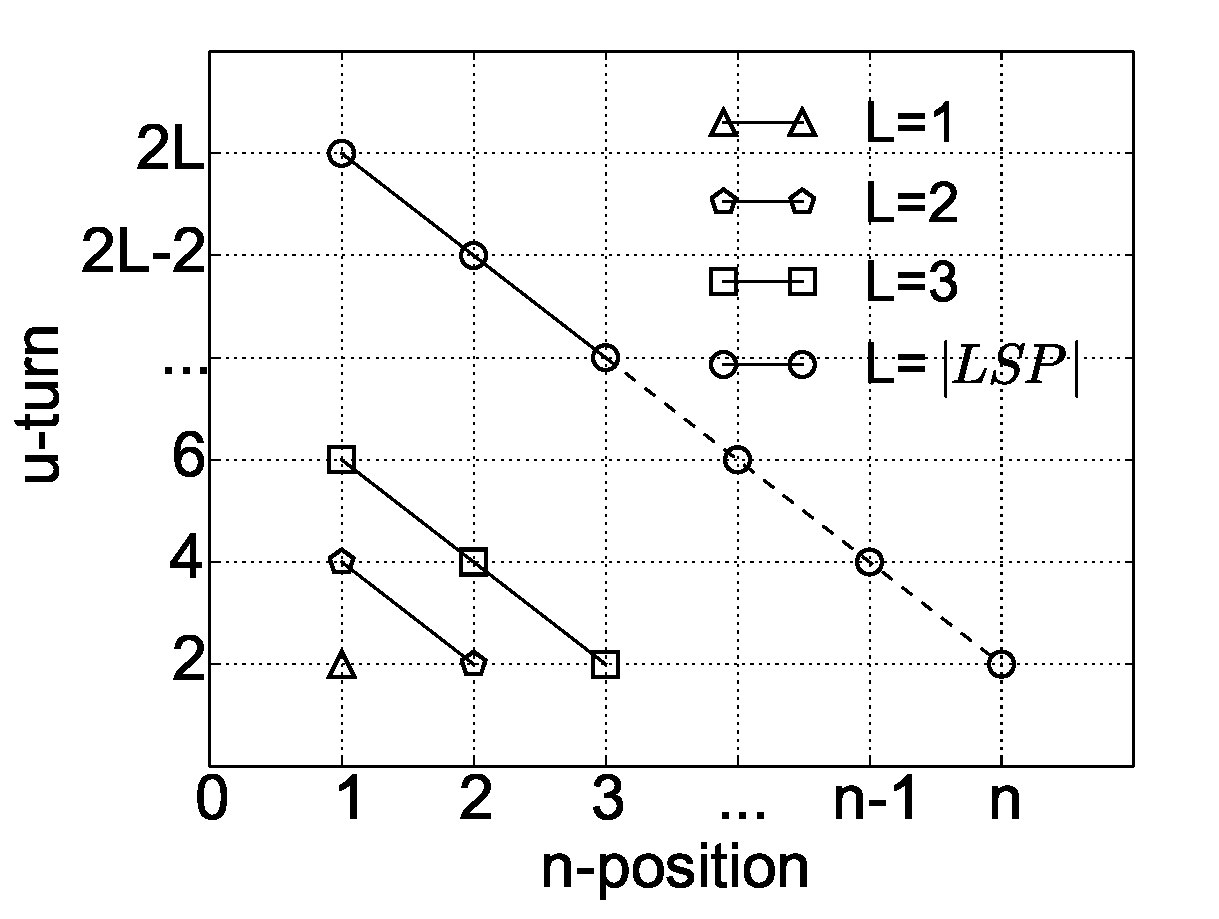
\includegraphics[width=4.5cm]{uturn1}}  
  \end{center}
\vspace{-0.5cm}  
  \caption{Signatures behavior for implicit MPLS tunnels.}
  \label{validation.signatures.fig}
\end{figure}

\begin{figure}[!t]
  \begin{center}
    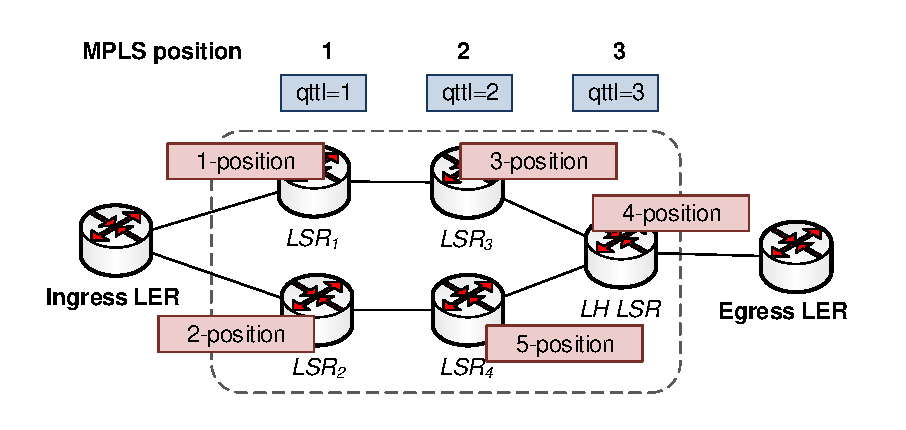
\includegraphics[width=8cm]{mpls_position}
  \end{center}
\vspace{-0.5cm}  
  \caption{Example of biased $n$-position. 
%  Our assumption consider that
%   $n$-position match with the real MPLS position. However, we need first to
%   verify this hypotesis in order to be sure that the behaviour shown on this
%   figure is not a common issue. 
  It shows a scenery where, due to per-packet load balancing issues on the
  Ingress LER, the $n$-position could be erroneously inferred: First,
  \traceroute reveals  $LSR_{1}$ (and associates it the $1$-position), the next
  \traceroute probe reveals the $LSR_{2}$ (and associates it the $2$-position)
  and so on.}
  \label{validation.MPLSpositionFig}
\end{figure}

In this section, we expose our methodology for validating the MPLS signatures
used to reveal implicit MPLS tunnels (see Sec.~\ref{related.revealing}).
Basically, we compare the LSR position within an MPLS tunnel, called the
\dfn{MPLS position}, with the different signatures values. Our main goal here is
to evaluate the u-turn accuracy.

The MPLS position of an LSR is obtained based on its appearance order in an LSR,
as revealed by \traceroute.  The appearance order is called \dfn{$n$-position},
i.e., The first LSR revealed by a \traceroute probe should be the first LSR
within the LSP ($1$-position) , the LSR revealed by the next consecutive
traceroute probe should be the second LSR within the LSP ($2$-position), etc.
Given that MPLS tunnels can be configured to perform load balancing (this is
quite common, as shown by Vanaubel et al.~\cite{Vanaubel15}), the $n$-position
revealed by \traceroute might lead to a bias with respect to the actual MPLS
position. This is illustrated in Fig.~\ref{validation.MPLSpositionFig}.

% Theorically, given an LSR, we could get its MPLS position through either its
% qTTL or its u-turn signature. Then, knowing the qTTL value of the LSR we can
% validate its u-turn signature (if any) or vice versa. However, on LSRs revealed
% only through u-turn signatures, qTTL values are not present so we need another
% way to know the related MPLS position. Thereby, we assume that the MPLS position
% could be obtained independently of the signatures values. Thus, we obtained the
% MPLS position based on the appearance order that an LSR is revealed by
% \traceroute and we call to this value $n$-position, i.e., The first LSR revealed
% by a \traceroute probe should be the first LSR within the LSP ($1$-position) ,
% the LSR revealed by the next consecutive traceroute probe should be the second
% LSR within the LSP ($2$-position), etc. Initially, we consider this just as an
% hypothesis because we do not know exactly the MPLS tunnel behaviour in regards
% with load balancing or others unexpected issues, i.e, unexpected load balancing
% behaviour could cause that the appearance order by an LSR in the traceroute
% ($n$-position) is biased in respect to the real MPLS position (see
% Fig.~\ref{validation.MPLSpositionFig}).

Implicit tunnels are based either on qTTL or u-turn signatures. Both of them are
directly related with MPLS position.  Indeed, first, the qTTL value refers to
the IP-TTL of the \echorequest packet when it enters the MPLS tunnel.
Therefore, a qTTL of $n$ in the resulting ICMP \ttlexceeded means that the sent
probe expired $n$ hops later than the Ingress LER of the LSP, i.e., an LSR reply
with qTTL$=n$ means that the LSR appears in the \dfn{$n$-position} in the LSP.
This is illustrated in Fig.~\ref{validation.qTTLFig}.  From the Ingress LER, the
qTTL starts to grow linearly with the LSP length.  We therefore expect observing
a qTTL=$1$ on the first LSR in the LSP, a qTTL$=2$ on the second LSR in the LSP,
etc.  Second, a u-turn value is related to the tunnel length, $L$, and the
$n$-position of the LSR within the tunnel (see Sec.~\ref{related.revealing}) as
is shown on Fig.~\ref{validation.uturn1Fig}.

\subsection{qTTL Signature}\label{validation.qttl}
%%%%%%%%%%%%%%%%%%%%%%%%%%%
\begin{figure}[!t]
  \begin{center}
    \subfigure[Tunnel length distribution]{\label{hist_length}
      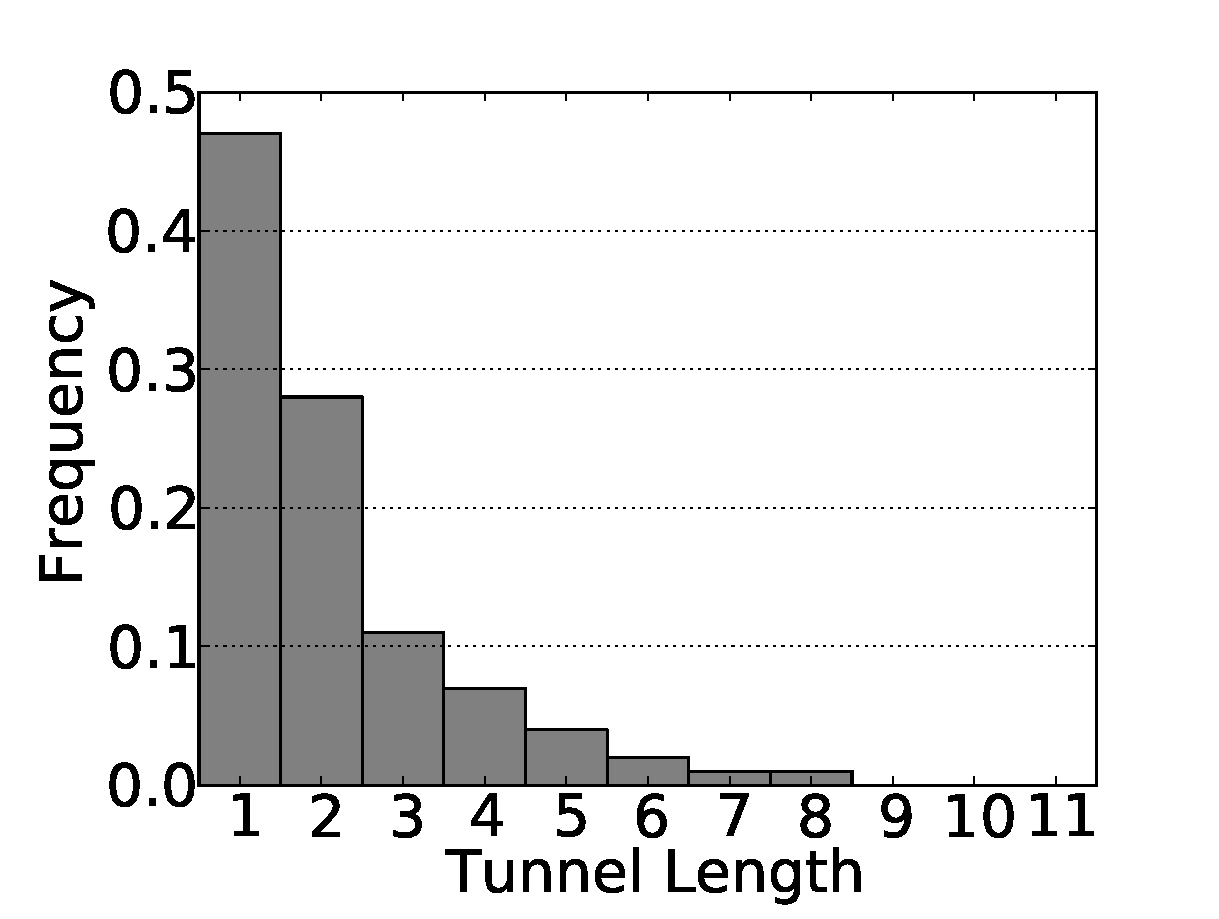
\includegraphics[width=4.3cm]{hist_length}}
\hspace{-0.3cm}      
    \subfigure[qTTL and $n$-position comparison]{\label{n_vs_qttl}
      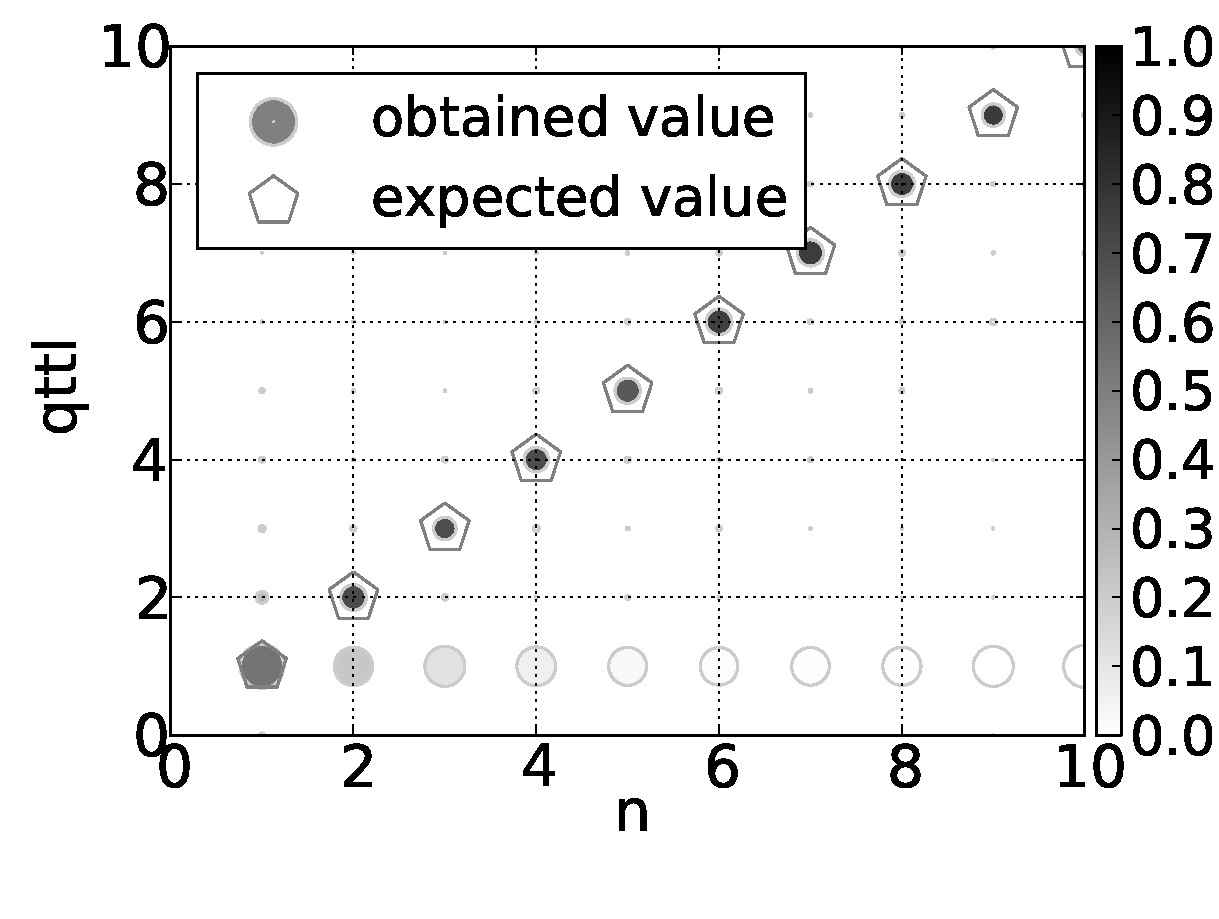
\includegraphics[width=4.3cm]{n_vs_qttl}}  
  \end{center}
\vspace{-0.5cm}  
  \caption{Comparison between obtained and expected values for qTTL and u-turn.}
  \label{validation.qttl.fig}
\end{figure}

Our signature validation relies on the hypothesis that the actual MPLS position
matches with the $n$-position, i.e., the $n$-position of the LSR within the LSP
corresponds to the qTTL value generated by that LSR. Said differently qTTL =
$n$.

In order to validate this assumption, we use the dataset described in
Sec.~\ref{dataset} and compare the qTTL with $n$-position for explicit and
implicit tunnels
% \ed{We compare also with explicit tunnels, the exact filter is: RFC4950 IS ON
% OR QTLL>1. Mainly, we do this in order to add information realted with the
% amount of those explicit tunnels with have QTTL and those who dont (QTTL=1)}.
The results are shown in Fig.~\ref{validation.qttl.fig}.  In particular,
Fig.~\ref{hist_length} provides the MPLS tunnel length distribution computed as
the number of LSRs in the tunnel.  We observe, confirming so previous
studies~\cite{SOM11,Vanaubel15,Donnet12}, that most of tunnels are rather short
(length $< 3$ in more than 80\% of the cases).

Fig.~\ref{hist_length} also provides, by extension, possible values for qTTL
(X-axis).  This suggests thus that qTTL values should oscillates between 1 and
8, with a strong predominance for short values (i.e., between 1 and 3). 

Fig.~\ref{n_vs_qttl} represents a scatter plot showing the relations between the
qTTL (Y-axis) and the $n$-position (X-axis).  The circle size in the scatter
plot is related with the occurrence frequency of Y-axis values regarding each
$n$-position.  The transparency of the circle is related with occurrence
frequency of the $n$-position regarding each Y-axis value.  For instance, on
Fig.~\ref{n_vs_qttl} for values where $n>1$, the biggest circles are mainly
located on qTTL$=1$ and qTTL=$n$.  So, this suggests that, for a given
$n$-position, the qTTL value usually takes either the value $1$ or $n$.

However, we notice, on Fig.~\ref{n_vs_qttl} that the qTTL signature highly
matches with $n$.   The bias $\textit{qTTL}=n \pm \epsilon$ could occur due to
two causes: one is the limitation in our method to reveal the first LSR in the
LSP when RFC4950 is not implemented (by definition of implicit tunnel); and the
second cause could occur due to load balancers (using Paris traceroute should
avoid load balancing issues, except for ``per packet'' load balancers).
In the later case, the \traceroute probes may follow different paths, as suggest
Fig.~\ref{validation.MPLSpositionFig}. Fig.~\ref{n_vs_qttl} also shows that qTTL
frequently takes the value of $1$, even for $n>1$, which means that the LSR
implements the RFC4950 but do not mach with the qTTL signature. 

We also find that around $2\%$ of LSRs do not react to qTTL signature, even if
their neighbors does, i.e., some LSRs interfaces located at $i_{n \pm 1}$
tunnel positions react properly to qTTL signatures but the LSR interface located
at $i_n$ position does not.

Nevertheless, the $n$-position is highly reliable and therefore, the potential
load balancer presence on LSPs is not a common issue. Indeed, we find that in
$58\%$ of the cases the $n$-position matches with the qTTL value while in
$36,3\%$ of cases the qTTL signature is not present on explicit tunnels and
takes the value of $1$, and just $6,7\%$ of the cases presented have some bias
around the expected value $n$. Those results support our hypothesis: the  MPLS
tunnel position highly matches with the $n$-position. Thereby, we use
$n$-position as a reference value to validate the u-turn signatures.

\subsection{u-turn Signature}\label{validation.uturn}
%%%%%%%%%%%%%%%%%%%%%%%%%%%%%%
\begin{figure}[!t]
  \begin{center}    
    \subfigure[u-turn on LSRs revealed through RFC4950 and qTTL]{\label{fig_uturn_a}
      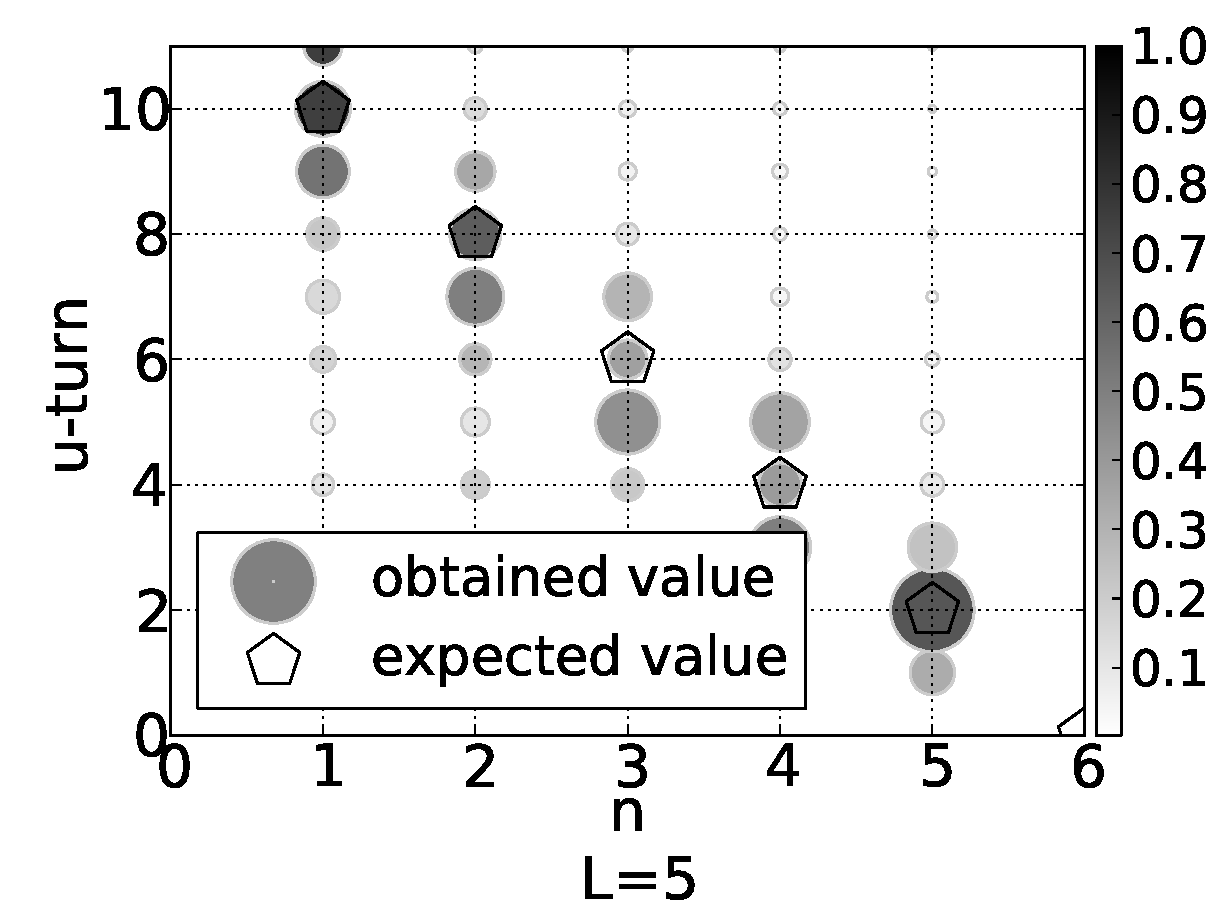
\includegraphics[width=4.3cm]{n_vs_uturn_L5_exp}}
\hspace{-0.3cm}      
    \subfigure[u-turn on LSRs where no other signature was found]{\label{fig_uturn_b}
      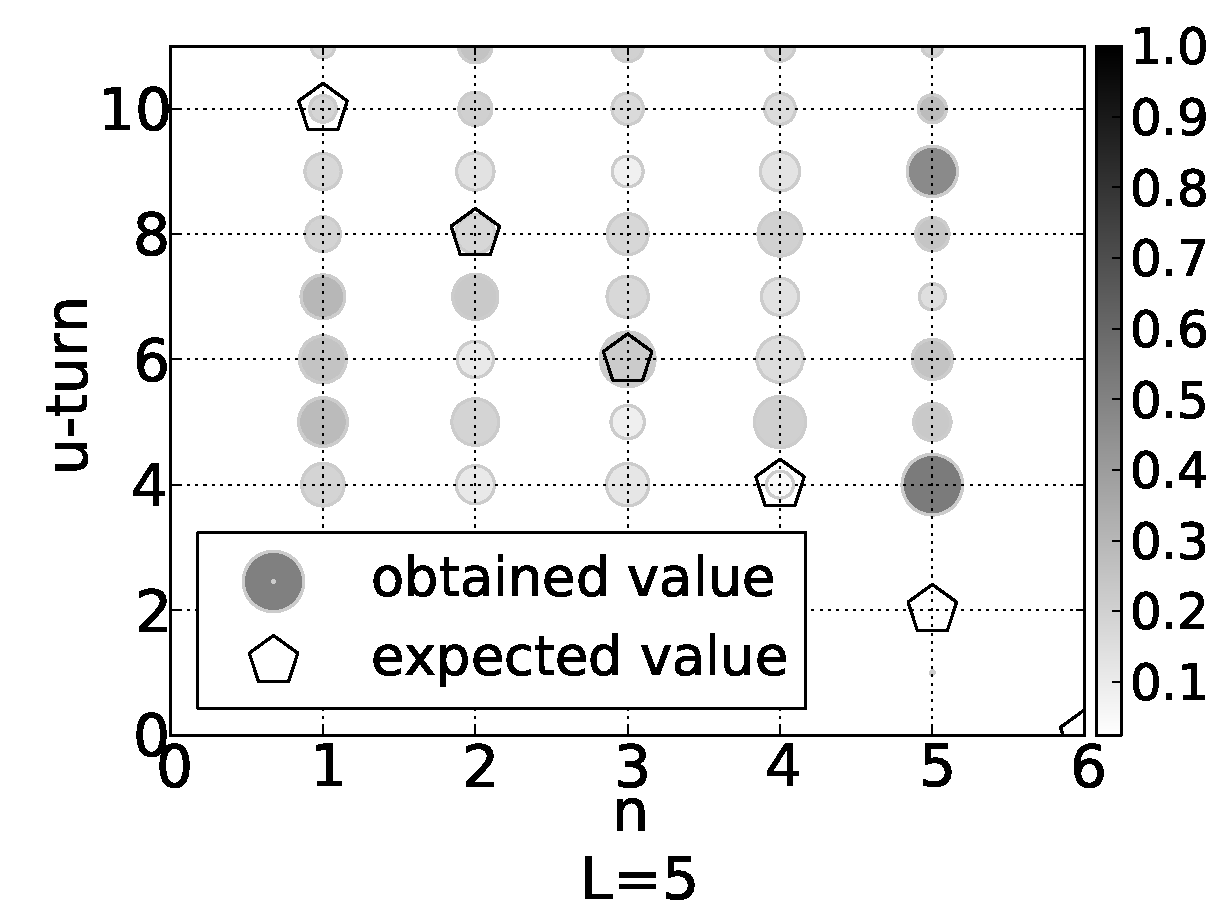
\includegraphics[width=4.3cm]{n_vs_uturn_L5}}
  \end{center}
\vspace{-0.5cm}  
  \caption{Comparison between obtained and expected values for u-turn
  signature.}
  \label{validation.uturn.fig}
\end{figure}

As explained in Sec.~\ref{related.revealing},  the expected u-turn value is of
the form $[2L, 2L-2, 2L-4,..., 2]$ where $L$ is the tunnel length and the array
position corresponds to the LSR position within the LSP, i.e., $n$ (see
Fig.~\ref{validation.uturn1Fig}).  The relationship between $L$, $n$, and the
expected value can thus be written as follows:
\begin{equation}
u-turn = 2 \times (L - (n-1)) .
\label{eqn.uturn}
\end{equation}

Because u-turn is commonly present in almost all LSRs, first, we compare $n$
with u-turn on LSRs revealed either explicitly or qTTL-based using the dataset
presented in Sec.~\ref{dataset} (Fig.~\ref{fig_uturn_a}). We also study 
$n$ value on LSRs where u-turn was the only detected signature
(Fig.~\ref{fig_uturn_b}). We use the filter $\text{u-turn}>3$ (i.e., avoiding
short tunnels where bias are more likely to appear) to avoid false positives.

The results for a given tunnel length $L=5$ are shown on
Fig.~\ref{validation.uturn.fig}, a scatter plot that must be read the same way
as Fig.~\ref{n_vs_qttl}.  Quickly said, Fig.~\ref{validation.uturn.fig} suggests
that u-turn is usually overestimated. Similar results where observed for other
tunnel lengths. 

We notice that obtained u-turn values are close to expected ones when the LSR
was either explicitly revealed or when qTTL is present (Fig.~\ref{fig_uturn_a}).
However, for LSRs revealed only by u-turn signatures (Fig.~\ref{fig_uturn_b})
the obtained and expected u-turn values commonly do not match. If we accept a
bias of $ \pm 2$ around the expected u-turn value over the entire of our
dataset, we notice that, on LSRs
explicitly revealed or qTTL based, the $60\%$ of obtained u-turn signatures
match with the expected values. However, for LSRs revealed only trough u-turn
signature, the obtained u-turn signature just match in less than $25\%$  with
the expected values.

Therefore, LSRs revealed only through u-turn are highly inaccurate, mainly,
because MPLS tunnels are not the only responsible for u-turn signature. Indeed, it is
also related with load balancing on the return path, where ICMP \echoreply and
ICMP \ttlexceeded at different hops may be load balanced~\cite{BRICE06}. 

%  but it is also related with load balancing issues in the return path.
% Basically, the two kinds of messages related with u-turn signatures (ICMP \echoreply  and
% ICMP \ttlexceeded) belong to diferents balancing \textit{flows} and thereby
% follow different return paths \cite{BRICE06}.

%is common for paths between the same pairs
%source-destination \cite{BRICE07}. This issue is called \dfn{per-flow} load
%balancing. Basically, packets that belongs to the same \dfn{flow} are treated
%similarly \cite{BRICE06}. A flow is identified by the first 32 bits of the IP
%\textit{payload}, e.g., TCP header. In the case of ICMP messages, this fields
%refers to \texttt{Type}, \texttt{Code}, and \texttt{Checksum}.
%By definition, u-turn signature is based on two kinds of ICMP messages:
%ICMP \echoreply \texttt{Code 11} and ICMP \ttlexceeded \texttt{Code 0}.
%Due to different codes for each ICMP message, there is no way to assure that
%they belong to the same flow identifier and thereby to be sure that u-turn value
%is caused just by MPLS tunnels.  \ed{The full explanation of ``per flow'' is not
%required (we can assume people are familiar with this).  But we have to clearly
%state that this is during the ``return'' path (i.e., from the LSR generating the
%\ttlexceeded towards the VP) that those per-flow LB can mainly occur.
%Otherwise, I miss something here.}
